\section{Escalation}

\begin{figure}[H]
	\centering
	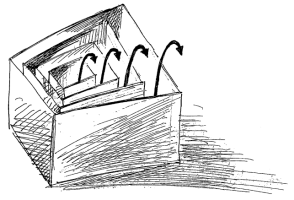
\includegraphics[width=\textwidth]{content/faulttolerance/images/escalation.png}
	\caption{escalation}
\end{figure}

\subsection{Problem}

Trotz allen Versuchen kann es sein, dass sich das System im Fehlerfall nicht wiederherstellen kann. Sowohl Correcting Audits, als auch Restarts, Data Resets und Rollback- oder Rollforwardversuche verlaufen manchmal erfolglos. In einigen Fällen kann es genügen, diese Versuche wiederholt anzuwenden, bis das gewünschte Ergebnis erzielt ist. Doch wie bei einer beschädigten LP, die immer wieder dieselbe Stelle wiederholt, ist manchmal drastischeres Eingreifen gefragt. Da das System das Prinzip von Minimize Human Intervention verfolgt, soll es dafür aber selbst verantwortlich sein.

\subsection{Lösung}

\textbf{\textbf{Wenn Fehlerkorrektur und -abschwächung fehlschlagen, führe die nächst drastischere Massnahme aus.}}

Es kann nützlich sein, einen Zähler zu haben, damit das System weiss, wie oft ein Wiederherstellungsversuch in welcher Zeit schon fehlgeschlagen ist. Wird ein gewisser Wert überschritten, kann die Eskalation in die nächste Phase ausgelöst werden.

\subsubsection*{Menschliches Eingreifen}

Ab einer bestimmten Phase wird menschliches Eingreifen unumgänglich. Dem Operator muss dann aber eine Liste mit möglichen Schritten vorliegen. Diese sollte so geordnet sein, dass zuerst Massnahmen ausgeführt werden, welche eine hohe Recoverywahrscheinlichkeit haben, aber gleichzeitig schnell sind und einen minimalen Einfluss auf andere Systemoperationen haben. Später folgen dann die schwereren Geschütze.

